% Created: 2019-12-10
% Plot participant data
% http://github.com/zhaobn/magic_stones

\documentclass{article}
\title{[Magic Stones] Report for Experiment 1}
\author{Bonan Zhao (b.zhao@ed.ac.uk)}

% Text formats: margin, font, spacing
\usepackage[margin=0.8in]{geometry}
\usepackage{charter}
\renewcommand{\baselinestretch}{1.3}

% Graphics
\usepackage{graphicx}
\usepackage{subcaption}
\graphicspath{{../figs/}}

\usepackage{amsmath}

\begin{document}
\maketitle

% Raw participant data
\section{Participant data}

\begin{figure}[h!]
	\centering
  \begin{subfigure}[t]{0.32\textwidth}
  	\centering
  	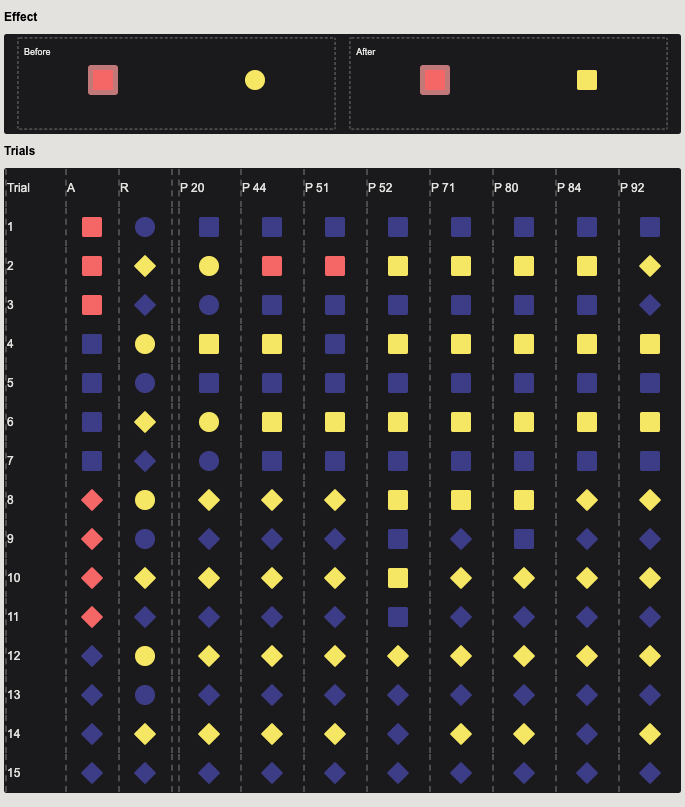
\includegraphics[width=\linewidth]{learn01} 
  	\caption{To the same shape} \label{fig:learn01}
  \end{subfigure}
  \hfill
  \begin{subfigure}[t]{0.32\textwidth}
  	\centering
  	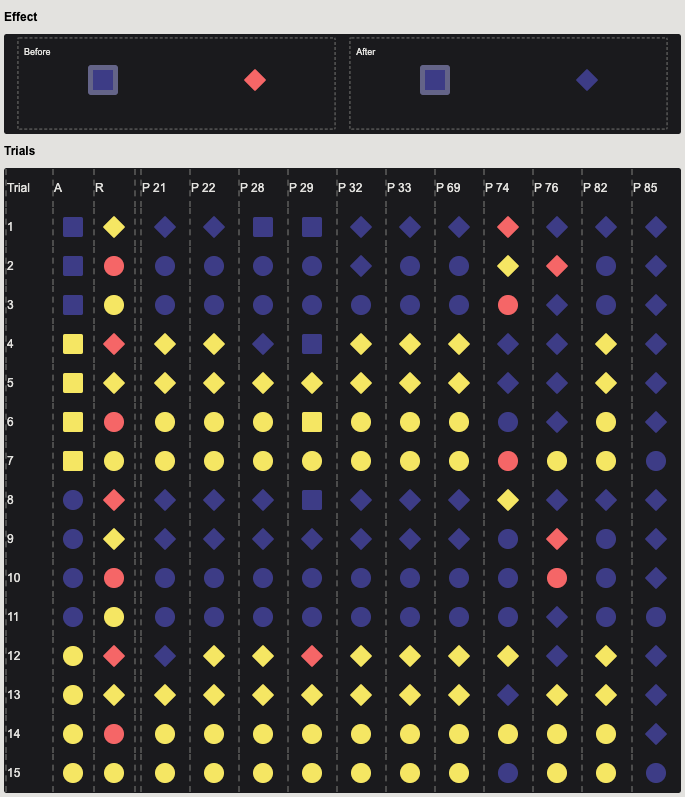
\includegraphics[width=\linewidth]{learn03} 
  	\caption{To the same color} \label{fig:learn03}
  \end{subfigure}
  \hfill
  \begin{subfigure}[t]{0.32\textwidth}
  	\centering
  	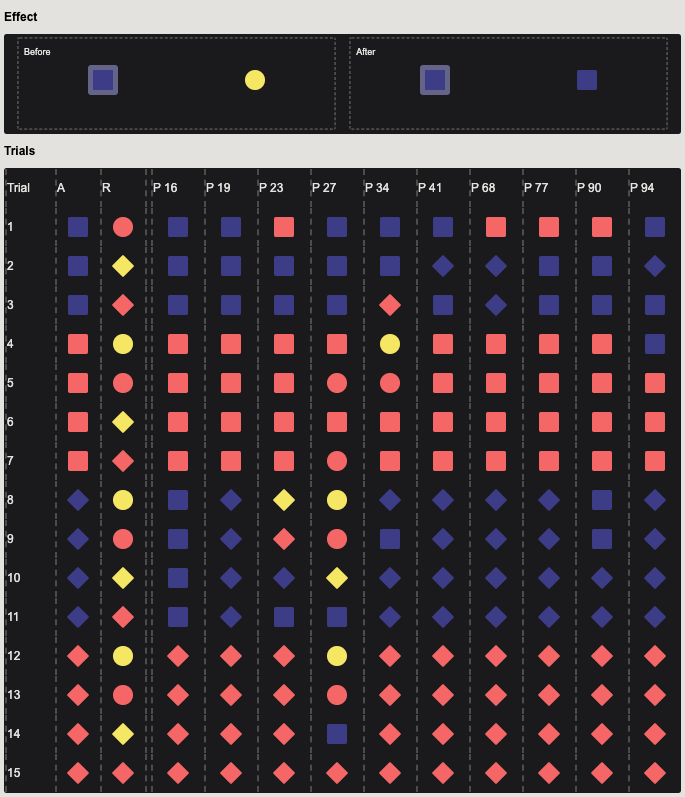
\includegraphics[width=\linewidth]{learn06} 
  	\caption{To the same object} \label{fig:learn06}
  \end{subfigure}

  \vspace{1em}
  \begin{subfigure}[t]{0.32\textwidth}
  	\centering
  	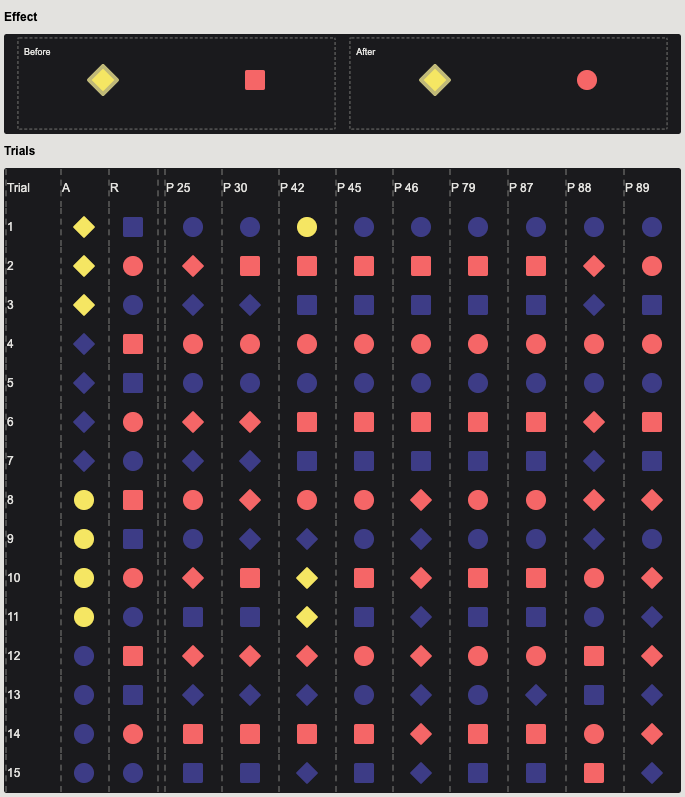
\includegraphics[width=\linewidth]{learn02} 
  	\caption{To a different shape} \label{fig:learn02}
  \end{subfigure}
  \hfill
  \begin{subfigure}[t]{0.32\textwidth}
  	\centering
  	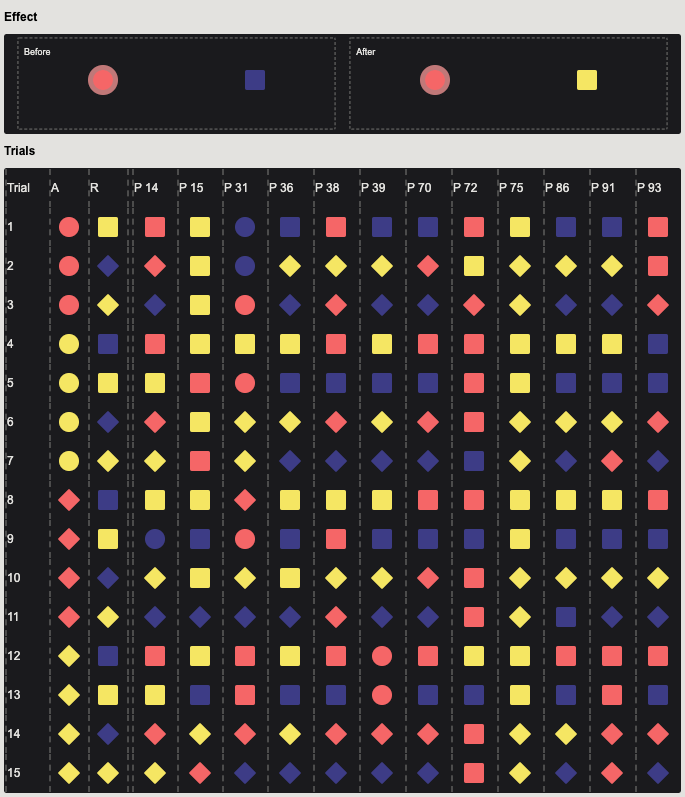
\includegraphics[width=\linewidth]{learn04} 
  	\caption{To a different color} \label{fig:learn04}
  \end{subfigure}
  \hfill
  \begin{subfigure}[t]{0.32\textwidth}
  	\centering
  	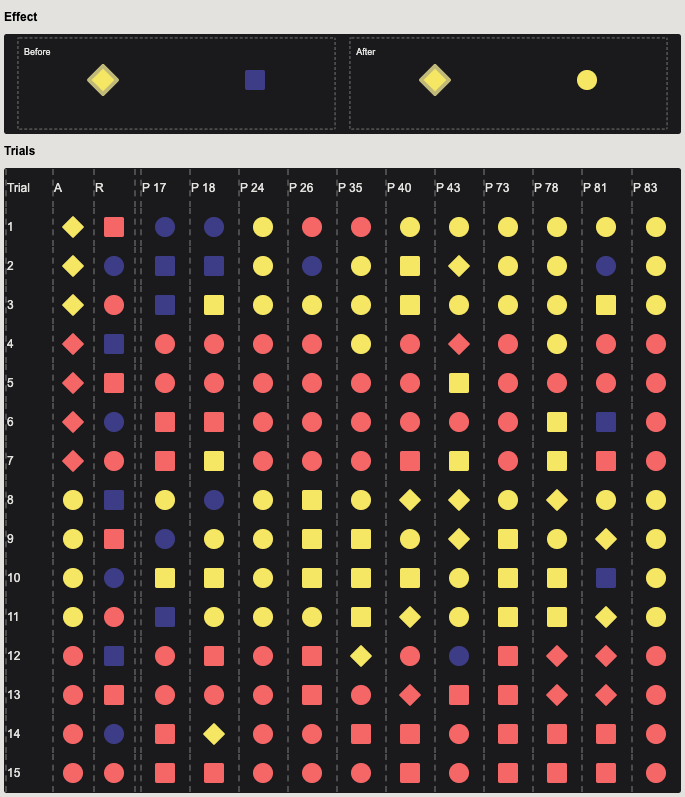
\includegraphics[width=\linewidth]{learn05} 
  	\caption{To a different object} \label{fig:learn05}
  \end{subfigure}
  \caption{Each figure is for one learning condition. 
  Each learning condition has 15 trials (15 rows).}
\end{figure}

\section{Stats}

\begin{itemize}
  \item Age: min 24, max 67, mean 41.1639, sd 11.1238 
  \item Gender: female 28 (45.9\%), male 33 (54.1\%)
  %\item Task duration (minutes): min 2.2068, max 10.0976, mean 4.8756, sd 1.8663
  %\item Self-report difficulty: min 0, max 10, mean 4.6557, sd 3.1564
\end{itemize}

\begin{table}[h!]
  \centering
  \begin{tabular}{c|l|c|c|c|c|c}
  Condition & Description & Count & Share & Task dur. mean (min.) & S-Dfty. mean & Variation \\
  \hline
  1        & To the same shape     & 8     & 13.11\% & 5.1873 & 3.38 & 10.83\% \\
  2        & To a different shape  & 9     & 14.75\% & 5.0942 & 7.89 & 18.33\% \\
  3        & To the same color     & 11    & 18.03\% & 4.7480 & 3.45 & 22.50\% \\
  4        & To a different color  & 12    & 19.67\% & 4.1504 & 5.17 & 38.33\% \\
  5        & To a different object* & 11    & 18.03\% & 5.2803 & 5.09 & 30.00\% \\
  6        & To the same object    & 10    & 16.39\% & 5.0351 & 3.00 & 16.67\% \\
  7        & Diff color + diff shape & 9    & - & 6.89 & 5.44 & 45.83\% \\
  \hline
  Total (ex. 7)    &                       & 61    &         & 4.8756 (sd 1.87) & 4.65 (sd 3.16) & \\
  \end{tabular}
  \caption{Basic stats per condition. S-Dfty.: Self-report difficulty.
  *: Same color + diff shape.}
  \label{table:conditions}
\end{table}

\subsubsection*{Variation}

Variation is defined as how much observed difference out of the maximal possible difference.
%
For a condition $C$ and each of its generalization task $i$, let $U_i$ be the number of unique predictions all participants made in this task, and $n$ be the number of participants, \emph{observed difference} is defined as $U_i - 1$ because of the intuition that if all the participants make the same prediction, the number of unique selections is 1 and variation should be 0, and \emph{maximal difference} $M_i$ is given by

\[M_i=
  \begin{cases}
    8 & \text{if } n \geq 9 \\
    n & \text{otherwise}
  \end{cases}
\]

Formally, variation measure $V_C$ for condition $C$ is $$V_C := (\sum_{i \in C}U_i-1)/\sum_{i \in C}M_i$$.

Overall, participants make quite homogeneous predictions - variation measure for all the conditions are below 40\% of the largest variations, with condition 4 (to a different color) being the one with most various predictions. For condition 1 (to the same shape), participants make very uniform predictions, with a variation measure of just 10.84\%.

\subsubsection*{``To the same xx'' V.S. ``To a different xx''}

Conditions 1, 3, and 6 can be classified as ``to the same xx'' group, where xx can be color, shape, or both (equivalent to the object), and conditions 2, 4, 5 can be classified as ``to a different xx'' group. Statistical test shows that compared to the ``to a different xx'' group, participant report the ``to the same xx'' group is significantly easier ($p<0.0001$), and make more homogeneous predictions ($p=0.0001$). However there is so significant difference for task duration between these two groups.

\section{Compliance}

A task \emph{complies} with the underlying rule if the selected stone is covered by predictions generated by the rule. 

Per condition aggregation shows that compliance goes in line with homogeneity - \texttt{learn01} has the highest compliance and lowest variation, \texttt{learn04}, on the other extreme, has the lowest compliance and highest variation.

As for each generalization task, task 5 has the highest compliance while 2, 8, and 9 has the lowest compliances. Task 2 is when the participant encounter a complete different normal stone for the first time, and for task 8, 9 participants face a complete different magic stone for the first time. Task 5 has a very specific setting: the magic stone and normal stone in this task have the same shape configurations as in the learning condition, and the magic stone and normal stone in this task have the same color - color that is different from both the magic stone and normal stone in the learning condition.

There is no correlation between individual compliance performance and participant age or gender.

\begin{figure}[h!]
  \centering
  \begin{subfigure}[t]{0.45\textwidth}
    \centering
    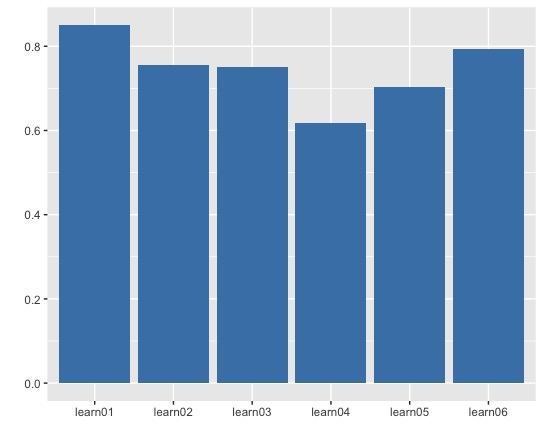
\includegraphics[width=\linewidth]{com_group} 
    \caption{Aggregated by conditions.}
  \end{subfigure}
  \begin{subfigure}[t]{0.45\textwidth}
    \centering
    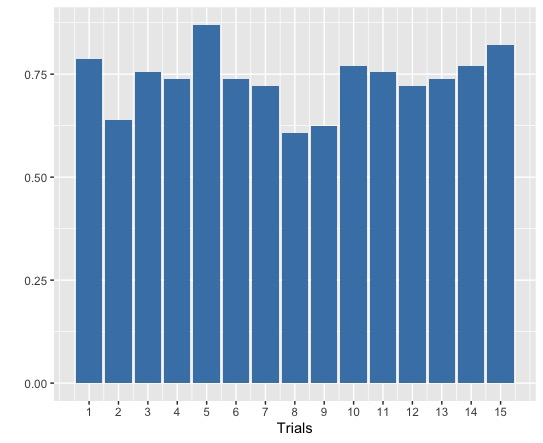
\includegraphics[width=\linewidth]{com_trial} 
    \caption{Aggregated by tasks.}
  \end{subfigure}

  \begin{subfigure}[t]{0.9\textwidth}
    \centering
    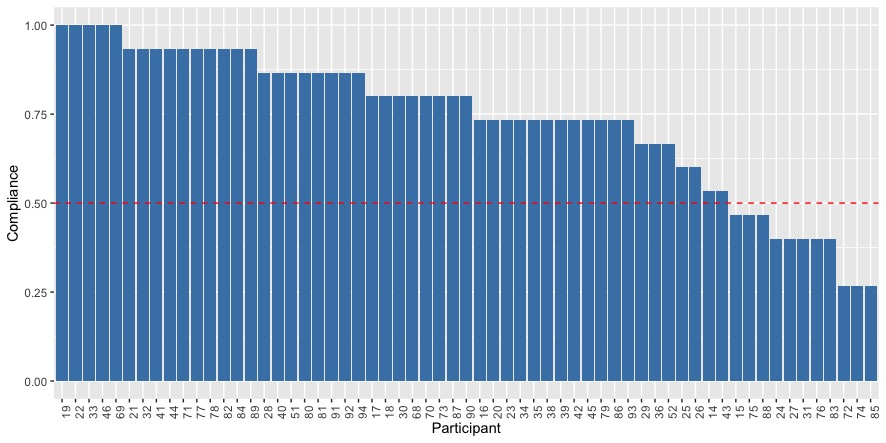
\includegraphics[width=\linewidth]{com_ind} 
    \caption{Individuals}
  \end{subfigure}
  \caption{Percent of selections that comply with the underlying rule.}
  \label{fig:compliance}
\end{figure}

\section{Theories}

Recall the nine theories in previous notes, as listed in Table~\ref{functions}. Figure~\ref{fig:theory_comp} shows to what extent these nine theories predict the underlying rule or participant data separately.

Each cell is a summary of how well a theory predicts all the tasks for one condition, call it $A$ (for \emph{agreement}). For the ``code setup'' group, $A_C = N_C/15$ where $N_C$ is the number of theory predictions that agree with condition $C$'s underlying rule. When comparing with participant data, for each selection $s$ in the theory predictions $TP$ and participant selections $PP$, $A_C = (\sum_{i \in C}|P_{TH}(s_i) - P_{PP}(s_i)|)/15$.


\begin{table}
  \centering
  \begin{tabular}{rrrrrrrrrr}
    Arrow & $o \rightarrow o$ & $o \rightarrow c$ & $o \rightarrow s$ & $c \rightarrow o$ & $c \rightarrow c$ & $c \rightarrow s$ & $s \rightarrow o$ & $s \rightarrow c$ & $s \rightarrow s$ \\
    \hline \hline
    $|f|$ & 81  & 27  & 27  & 27  & 9   & 9   & 27  & 9   & 9   \\
    \hline
    Total &     &     &     &     &     &     &     &     & 225
  \end{tabular}
  \caption{Number of causal power functions each arrow combination produces. $o$: $object$, $c$: $color$, $s$:$shape$.}
  \label{functions}
\end{table}

\begin{figure}[h!]
  \centering
  \begin{subfigure}[t]{0.45\textwidth}
    \centering
    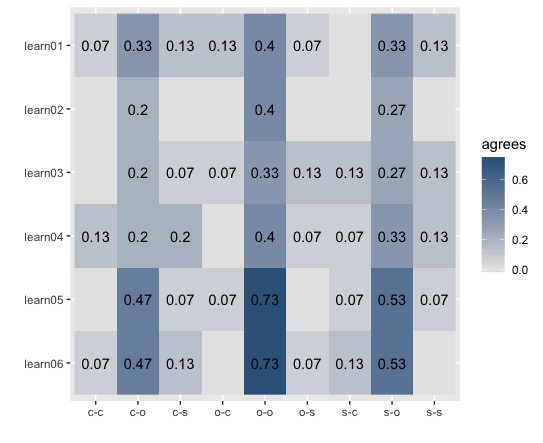
\includegraphics[width=\linewidth]{th_norm} 
    \caption{With code setup}
  \end{subfigure}
  \hfill
  \begin{subfigure}[t]{0.45\textwidth}
    \centering
    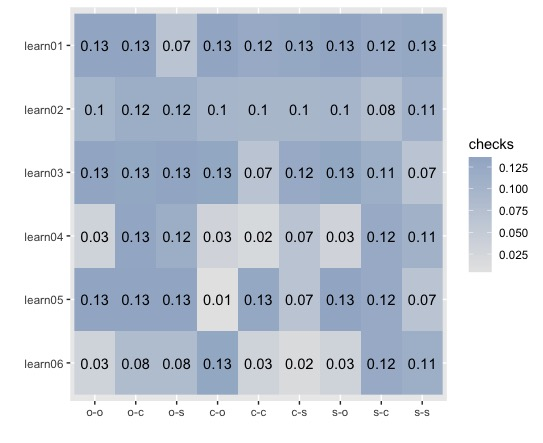
\includegraphics[width=\linewidth]{th_ppt} 
    \caption{With participant selections}
  \end{subfigure}
  \caption{Theory predictions versus data.}
  \label{fig:theory_comp}
\end{figure}


\end{document}


